% =========================================================================
% When Does a Small Model Know to Hand Off?
% Zero-Training Escalation Gates for Full-Duplex Speech Models
%
% Draft v0.1 (2026-07-24) — generated from TECHNICAL_REPORT.md v3.
% Source of truth for numbers: interactive_paper/RESULTS.md (Phases 0-7a).
% Build: pdflatex + bibtex (Overleaf default works).
% \todonote{...} marks open items; the "TODO / Roadmap" section at the end
% collects experiment-level TODOs and must be deleted before submission.
% =========================================================================
\documentclass[11pt]{article}

\usepackage[margin=1in]{geometry}
\usepackage[T1]{fontenc}
\usepackage[utf8]{inputenc}
\usepackage{lmodern}
\usepackage{microtype}
\usepackage{amsmath,amssymb}
\usepackage{graphicx}
\usepackage{booktabs}
\usepackage{multirow}
\usepackage{caption}
\usepackage{xcolor}
\usepackage[round]{natbib}
\usepackage[colorlinks=true,linkcolor=blue!60!black,citecolor=blue!60!black,urlcolor=blue!60!black]{hyperref}

\graphicspath{{figures/}}

% ---- draft machinery ----------------------------------------------------
\newcommand{\todonote}[1]{\textcolor{red!80!black}{\textbf{[TODO: #1]}}}
\newcommand{\ptrue}{p(\mathrm{True})}
\newcommand{\auc}[1]{#1}

\title{When Does a Small Model Know to Hand Off?\\
\Large Zero-Training Escalation Gates for Full-Duplex Speech Models}

\author{%
Ruoyu He \and Jisen Li \and Changyi Yang \and Zetian Li \and Zhongzhu Zhou\\[0.6em]
\normalsize \todonote{affiliations, emails, author order + contribution footnotes}%
}
\date{Draft v0.1 --- \today}

\begin{document}
\maketitle

\begin{abstract}
Full-duplex speech models must answer in real time with a small on-device
backbone, yet many queries exceed that backbone's competence. We study the
first half of a two-stage design: can the small model itself signal, with
\emph{zero additional training}, that a query should be escalated to a large
cloud model? We attach candidate gate signals---decode-time scalars, linear
probes on hidden states, and verbalized self-evaluation
($\ptrue$)---to MiniCPM-o~4.5 (9B, omni/duplex fine-tune of Qwen3-8B) and
evaluate them against judged failure labels on 600 frozen public-benchmark
queries, with matched-pair controls across ten backbones and both text and
speech input. We find that (i) a standard final-layer probe is largely a
query-type shortcut that inverts under distribution shift, while pre-answer
$\ptrue$ catches 100\%-fail long-tail traps with no training; (ii) duplex
fine-tuning \emph{overwrites self-knowledge readouts without destroying the
underlying information}: mid-layer probe transfer is near the raw backbone's
(leave-one-pool-out math 0.931 at layer 22 vs.\ 0.366 at layer 35), and the
damage is specific to the late-layer last-token position where a streaming
head encodes turn control; (iii) the two readouts fail in complementary
modalities---the late-layer cliff is text-input-specific, whereas verbalized
introspection collapses on audio input because the verbal self-check runs
over text-token pathways that audio embeddings do not feed; (iv) the
modality-shared mid-layer core that makes cheap text-side calibration
transfer to speech is created by end-to-end training and is absent under a
frozen-backbone adapter. As a system, the resulting mid-layer gate decides in
20\,ms (text) / 45\,ms (audio)---before the first output token---and
gated-cloud escalation dominates the model's own thinking mode on both
accuracy and latency at every escalation rate (e.g.\ 0.787 vs.\ 0.637
accuracy at $3.4\times$ lower latency at a 33\% escalation budget).
We close the loop live: in full streaming duplex sessions, an
end-of-turn mid-layer read decides before the first output token
(AUC .887), the returned expert answer is spoken by the talker---the
same low-confidence state that fires the gate predicts relay compliance,
so escalation and injection are two uses of one signal---and the live
system climbs monotonically from its honest streaming floor
(.422 $\to$ .633 at 57\% escalation on speakable content), with the gap
to offline operation decomposed into measured audio, streaming, and
speech-channel taxes. Finally, the gate transfers \emph{frozen}: on six
public speech benchmarks it fires at sane rates with only label-free
threshold quantiles, lifts Speech TriviaQA to .860 live (official
offline anchor: .755; a 30B omni model: .629), matches the cloud expert
at half the expert calls on Llama Questions, and the mid-network
readability it exploits replicates on a second, architecturally
disjoint duplex family (hybrid-Mamba NemotronLabs-VoiceChat-11B) ---
evidence that duplex models as a class carry a free, readable
self-assessment signal that standard readouts miss.
\end{abstract}

\section{Introduction}
\label{sec:intro}

Voice assistants built on full-duplex speech models
\citep{defossez2024moshi,zeng2024glm4voice,xu2025qwen25omni} face a
structural tension. The conversational loop---listening while speaking,
turn-taking inside a $\sim$200--300\,ms budget
\citep{stivers2009universals}---demands a small, low-latency model close to
the user. Answer quality on knowledge- and reasoning-heavy queries demands a
large one. The natural architecture is a \emph{talker--thinker} split,
echoing the System~1/System~2 distinction \citep{kahneman2011thinking}: a
small duplex ``talker'' holds the live session and answers by default, and a
large cloud ``thinker'' is consulted only when needed. This paper is about
the load-bearing decision in that architecture: \textbf{when should the
talker hand off?}

We deliberately restrict ourselves to \emph{zero-training} gate signals ---
quantities that can be read off the small model as-is, without fine-tuning
it: decode-time scalars (entropy, margin), linear probes on hidden states
\citep{alain2017understanding}, and verbalized self-evaluation, i.e.\
$\ptrue$-style ``Would you answer this correctly?'' prompts
\citep{kadavath2022language}. The constraint is practical (duplex fine-tunes
are expensive and fragile to retrain) but it also sharpens the scientific
question: \emph{does a small full-duplex model already know what it does not
know, and can that knowledge be read out in time to act on it?}

Our answer, developed over a controlled study of ten
backbones/fine-tunes and both input modalities, is: \textbf{the knowledge is
there; the readouts are what break, and they break in systematic,
duplex-fine-tune-induced ways.} Concretely:

\begin{enumerate}
\item \textbf{Standard probes flatter to deceive (\S\ref{sec:rq1}).} A
  final-layer hidden-state probe reaches AUC 0.822, but an audit shows it is
  mostly a query-\emph{type} recognizer: a pool-identity oracle alone scores
  0.715, and leave-one-pool-out (LOPO) transfer \emph{inverts} on math
  (0.372). Pre-answer $\ptrue$ needs no training, beats the probe on most
  backbones, and scores 100\%-fail SimpleQA traps at 0.945 --- but only if
  asked \emph{before} the model answers; after answering, it endorses its own
  confident-wrong answer (0.945 $\rightarrow$ 0.360).
\item \textbf{Duplex fine-tuning overwrites readouts, not knowledge
  (\S\ref{sec:duplex}).} Across matched pairs (raw vs.\ omni-streaming vs.\
  duplex fine-tunes of the same backbone), LOPO probe transfer degrades in
  the order raw $>$ omni-streaming $>$ duplex, with label coverage
  controlled. A full layer$\times$position sweep localizes the damage: on
  MiniCPM-o~4.5, LOPO math is 0.931 at layer 22 but 0.366 at layer 35, with
  a sharp cliff over the last four layers, only at the last-token position
  --- exactly where a streaming head must encode turn-control state.
\item \textbf{Each readout has one blind modality (\S\ref{sec:speech}).}
  The late-layer cliff is text-input-specific: under audio input the final
  layer does not invert (0.936). Conversely, verbalized introspection
  collapses on audio input (trap $p_{\mathrm{yes}}$ $0.055 \rightarrow
  0.556$) on both MiniCPM duplex generations while omni-streaming and
  frozen-backbone controls stay intact. Three controlled arms (ASR audit,
  filler audio, audio+text duplication) pin the mechanism to \emph{binding}:
  the verbal self-check runs over text-token pathways that audio embeddings
  do not feed, while a probe reads the same information at 0.93+.
\item \textbf{End-to-end training creates the shared core
  (\S\ref{sec:speech}).} Text$\leftrightarrow$audio probe transfer is
  $\sim$0.86 on every end-to-end model but dead ($0.52$--$0.60$) on
  Freeze-Omni's frozen backbone with identical text weights --- so the
  practical recipe ``calibrate on cheap text, deploy on speech'' is valid
  for end-to-end models only.
\item \textbf{The gate wins as a system (\S\ref{sec:system}).} The mid-layer
  probe decides in 20\,ms (text) / 45\,ms (audio), before the first output
  token. Against the model's own \texttt{enable\_thinking} mode, gated-cloud
  escalation dominates on both accuracy and latency at every escalation
  rate, because the gate flags knowledge/trap failures that thinking cannot
  fix --- external escalation is \emph{necessary}, not merely better.
\end{enumerate}

\begin{figure}[t]
  \centering
  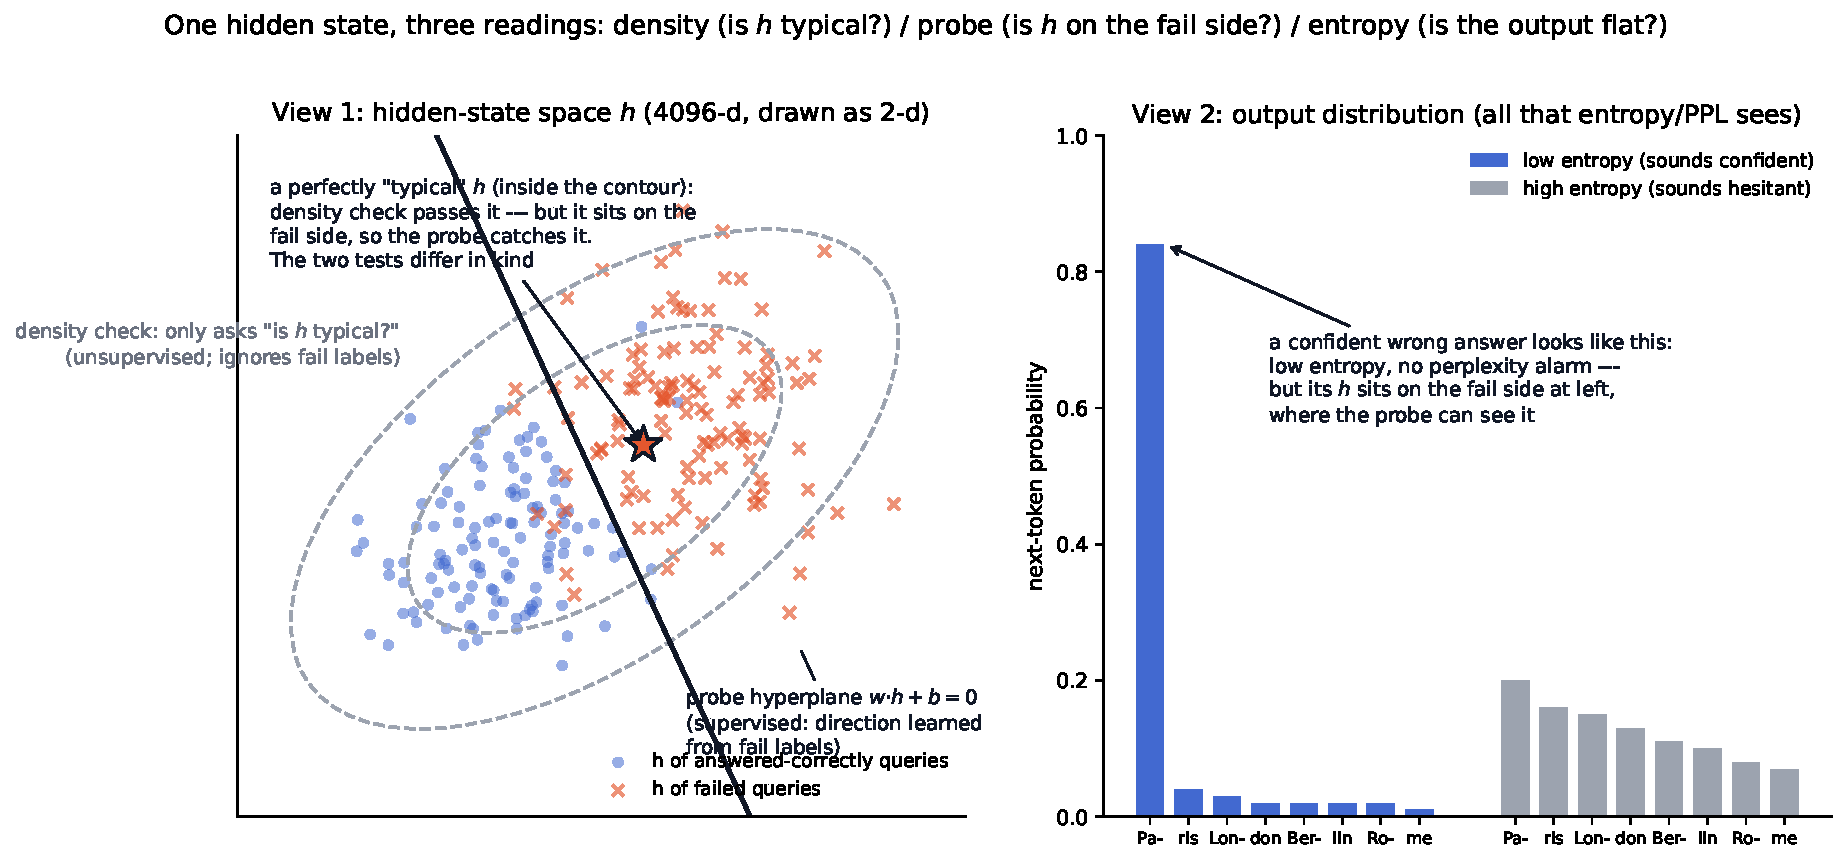
\includegraphics[width=\linewidth]{concept_probe_vs_ppl}
  \caption{Conceptual contrast between a supervised probe in hidden-state
  space and what output-distribution scalars (entropy/perplexity) can see.
  \todonote{regenerate this figure with English labels (current version has
  Chinese axis/legend text); source:
  \texttt{figures/concept\_probe\_vs\_ppl.py}}}
  \label{fig:concept}
\end{figure}

This is explicitly \textbf{step~1 of a two-step design}. Step~2 --- how the
thinker's result is returned into a live duplex session (injection protocol,
authority framing, stall phrases) --- is scoped but not solved here; our
streaming experiments already surface its first real obstacle (the talker
pushes back on injected results that conflict with its own reasoning,
\S\ref{sec:discussion}), and our overlap analysis (\S\ref{sec:system})
quantifies its timing budget.

\section{Related Work}
\label{sec:related}

\paragraph{Do language models know what they know?}
\citet{kadavath2022language} introduced $\ptrue$ and P(IK) self-evaluation
and showed large models are reasonably calibrated about their own answers;
\citet{lin2022teaching} trained models to verbalize uncertainty. A parallel
line reads correctness from internal states: linear probes
\citep{alain2017understanding} on hidden activations separate true from
false statements \citep{azaria2023internal,marks2024geometry}, latent
knowledge can be found without supervision \citep{burns2023discovering}, and
intermediate layers encode more truthfulness information than the output
distribution reveals \citep{orgad2024llms} --- consonant with our mid-layer
findings. Output-side uncertainty measures such as semantic entropy
\citep{kuhn2023semantic,farquhar2024detecting} require sampling multiple
generations, which a real-time duplex loop cannot afford. Our contribution
to this literature is not a new signal but a \emph{controlled account of
when the standard readouts break}: we show the probe and $\ptrue$ readouts
fail in complementary, modality- and architecture-specific ways under
duplex fine-tuning, while the underlying information survives.

\paragraph{Routing, cascades, and deferral.}
Cost-quality routing across LLMs is well studied: FrugalGPT
\citep{chen2023frugalgpt} cascades models with a learned scorer, HybridLLM
\citep{ding2024hybrid} trains a query router, RouteLLM \citep{ong2024routellm}
learns routers from preference data, and RouterBench
\citep{hu2024routerbench} standardizes evaluation;
\citet{llmrouterbench2026} report that many routers fail to beat simple
baselines under a unified protocol and attribute the remaining oracle gap to
model-recall failures. These routers decide from \emph{query-side} features
before generation, and the large model then answers the user directly. Both
assumptions fail in full-duplex voice: the user talks to one voice whose
session state (audio context, duplex KV cache) lives in the small model, and
our audit (\S\ref{sec:rq1}) quantifies exactly how far query-side features
go --- they are the ``type shortcut'' whose transfer collapses under
distribution shift, whereas the model-internal mid-layer signal transfers.
Classical learning-to-defer \citep{madras2018predict} and early-exit
computation \citep{schuster2022confident} are the same decision inside one
model; speculative decoding \citep{leviathan2023fast} inverts our roles
(large model verifies small drafts). Reasoning-mode escalation
(\S\ref{sec:system}) connects to test-time-compute models
\citep{guo2025deepseekr1}: we find self-escalation to a thinking mode is
dominated by external escalation because the flagged failures are
knowledge-bound, not compute-bound.

\paragraph{Full-duplex and omni speech models.}
End-to-end spoken dialogue models now span duplex designs --- dGSLM
\citep{nguyen2023generative}, Moshi with its Inner Monologue
\citep{defossez2024moshi}, GLM-4-Voice \citep{zeng2024glm4voice} --- and
streaming omni models such as Qwen2.5-Omni \citep{xu2025qwen25omni};
Freeze-Omni \citep{wang2024freezeomni} attaches speech adapters to a frozen
LLM, and Qwen2-Audio \citep{chu2024qwen2audio} covers audio-understanding
fine-tunes. Our target, MiniCPM-o~4.5
\citep{yao2024minicpmv,openbmb2026minicpmo}, is a 9B omni/duplex fine-tune
of Qwen3-8B \citep{yang2025qwen3}. We use this landscape as a
\emph{controlled independent variable}: matched pairs separating raw
backbones, audio-only fine-tunes, streaming-omni fine-tunes, duplex
fine-tunes, and frozen-backbone adapters let us attribute readout damage to
duplex-ness specifically, and the shared mid-layer core to end-to-end
training specifically.

\paragraph{Evaluation practice.}
Our query pools come from public benchmarks only: SimpleQA
\citep{wei2024simpleqa} for confidently-wrong long-tail traps (cf.\ PopQA
\citep{mallen2023popqa}), MMLU-Pro \citep{wang2024mmlupro}, TriviaQA
\citep{joshi2017triviaqa}, GSM8K \citep{cobbe2021gsm8k} and MATH-500
\citep{hendrycks2021math,lightman2024lets}, and Dolly/Alpaca instruction
data \citep{conover2023dolly,taori2023alpaca}. Adequacy labels come from an
LLM judge \citep{zheng2023judging} validated by a stronger re-judge
(agreement 0.962 text / 0.945 audio). The audio arm TTS-renders the frozen
pool, following the practice of Spoken-SQuAD \citep{li2018spokensquad} and
VoiceBench \citep{chen2024voicebench}; real-speech validation on SD-QA
\citep{faisal2021sdqa} is planned (\S\ref{sec:todo}).

\section{Experimental Setup}
\label{sec:setup}

\subsection{Models}
\label{sec:models}
The target model is MiniCPM-o~4.5 (9B; omni + full-duplex fine-tune of
Qwen3-8B), run in bf16 with greedy decoding and seed 42. To attribute
effects to the kind of fine-tune rather than the backbone, we assemble
ten models spanning raw backbones, a second duplex generation
(MiniCPM-o~2.6), a streaming-omni fine-tune (Qwen2.5-Omni-7B), an
audio-only fine-tune (Qwen2-Audio-7B), and a frozen-backbone adapter
model (Freeze-Omni, LLM weights byte-identical to its raw control);
the full roster is Table~\ref{tab:models} (appendix). The comparison
statistic is always the within-pair difference. All model checkpoints
remain frozen throughout; the escalation expert is \texttt{gpt-5.5} at
low reasoning effort.

\subsection{Dataset and labels}
\label{sec:dataset}
The internal dataset is 600 queries in five pools, frozen before any
gate experiment (360 calibration / 240 test): \emph{trap} = SimpleQA
\citep{wei2024simpleqa} (the target fails 100\%), \emph{hard-knowledge}
= MMLU-Pro \citep{wang2024mmlupro}, \emph{easy-fact} = TriviaQA
\citep{joshi2017triviaqa}, \emph{easy-chat} = Dolly/Alpaca
\citep{conover2023dolly,taori2023alpaca}, \emph{hard-math} = GSM8K tail
+ MATH-500 \citep{cobbe2021gsm8k,hendrycks2021math,lightman2024lets};
public benchmarks only, no LLM-generated queries. Adequacy labels come
from an LLM judge \citep{zheng2023judging} with structured outputs,
blind to the gate and validated by a stronger re-judge (agreement 96.2\%
text / 94.5\% audio; every headline number moves $\le$1 point under the
stronger labels). The audio arm renders the same frozen pool to speech
with single-voice TTS (content unchanged; only modality varies),
following Spoken-SQuAD / VoiceBench practice
\citep{li2018spokensquad,chen2024voicebench}. Judge prompts, pins, and
spend: Appendix~\ref{app:prompts}--\ref{app:repro}.

\subsection{Probe training and baseline signals}
\label{sec:signals}
We compare three signal families: (i) decode scalars: max token
entropy or margin over the first $k$ decode steps; (ii) linear probes:
logistic regression on hidden states, with layer and position selected
on calibration data; and (iii) verbalized self-evaluation
\citep{kadavath2022language}: $\ptrue$-pre asks ``would you answer this
correctly?'' before answering, $\ptrue$-post asks about a drafted
answer; $P(\text{Yes})$ is read from the first token's distribution.
The representation analyses use a single-position, 4096-d L22 probe
fit on the 360-query calibration split. The live system uses the same
layer plus two pooled positions, fit on a wider 2{,}310-query
calibration mix that is disjoint from the external benchmarks.
Concurrent and native serving change the read point, so those
validations refit the same feature set in regime; Appendix
\ref{app:signal} records the full calibration ledger.

\subsection{Benchmarks and evaluation protocol}
\label{sec:evalproto}
Audio-side findings are validated on real human recordings (SD-QA,
\citealp{faisal2021sdqa}); the frozen gate is evaluated on external
public speech benchmarks with their official audio
(\S\ref{sec:transfer}). In-distribution AUC is diagnostic, not the
main robustness claim, because query-pool identity is predictive in
the calibration mix. We therefore use LOPO AUC to test distribution
transfer and text-trained/audio-scored AUC to test modality transfer.
For the live system, the key comparison is against matched-rate random
escalation: an improvement over always-local operation can come from
the expert alone, while an improvement over random at the same call
rate measures the value of the gate's ranking.

\section{Which Signal Knows the Model Will Fail? (Text Input)}
\label{sec:rq1}

\subsection{Headline comparison}

Table~\ref{tab:rq1} compares the candidate signals on MiniCPM-o~4.5
(calibration split; probe numbers are 5-fold out-of-fold).
Figure~\ref{fig:roc} shows the ROC curves.

\begin{table}[t]
\centering\small
\caption{Signal AUCs against judged failure labels, MiniCPM-o 4.5, text
input. Bracketed interval is a bootstrap 95\% CI.}
\label{tab:rq1}
\begin{tabular}{lcc}
\toprule
signal & AUC & training needed \\
\midrule
$\ptrue$-post (post-draft) & \textbf{0.899} & none \\
probe on $h_{\text{prompt}}$ (final layer) & 0.822 [0.777, 0.863] & LR on calib \\
$\ptrue$-pre (pre-answer) & 0.807 & none \\
max entropy@4 (best decode scalar) & 0.696 & none \\
\bottomrule
\end{tabular}
\end{table}

\begin{figure}[t]
  \centering
  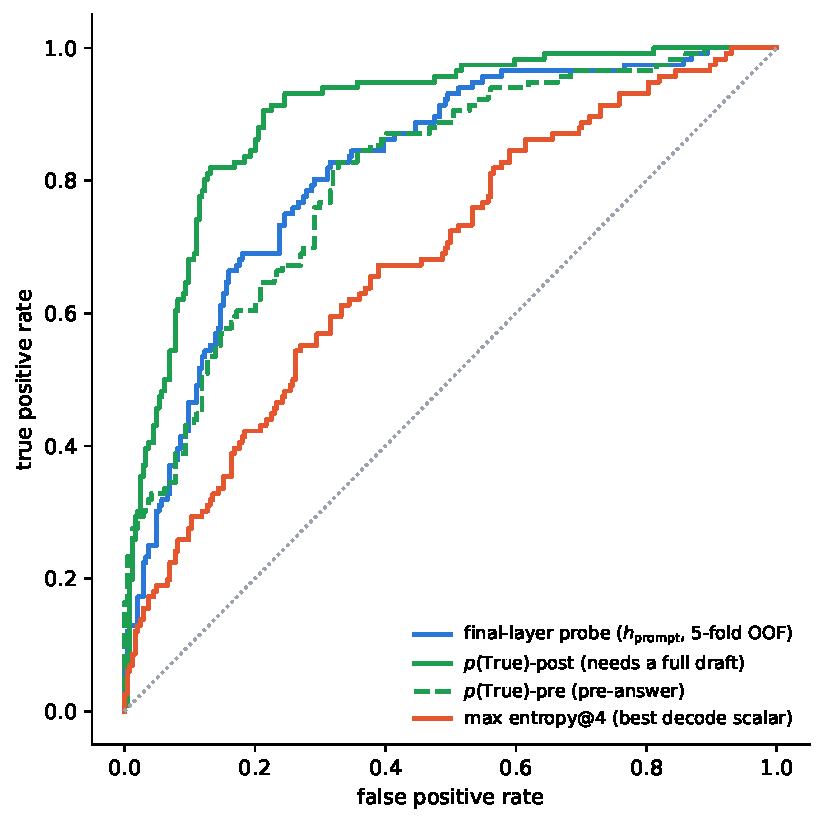
\includegraphics[width=.72\linewidth]{roc}
  \caption{ROC of the final-layer probe vs.\ decode scalars (calibration
  split). \todonote{regenerate to include the $\ptrue$ curves on the same
  axes}}
  \label{fig:roc}
\end{figure}

\subsection{The probe's number is a type shortcut}
\label{sec:audit}

The probe's 0.822 does not mean what it appears to mean. Three audit results
(all calibration-only): (i) the same hidden state classifies the
\emph{source pool} of a query at 95.8\%; (ii) a pool-identity oracle alone
--- predict each pool's base fail rate --- already reaches AUC 0.715; (iii)
appending true pool labels to the probe adds nothing (0.822 $\rightarrow$
0.821), i.e.\ the probe has already absorbed the type information. The
decisive test is leave-one-pool-out (LOPO) transfer: held-out math
\emph{inverts} to 0.372 --- the probe scores terse MATH-500 items as
``safer'' than verbose GSM8K items, a style-familiarity artifact --- and the
mean escalation score on the 100\%-fail trap pool is 0.232. Decode entropy
is $\approx$ chance on two of three raw backbones tested. In-distribution
AUC therefore overstates what a query-side signal knows; we treat LOPO as
the primary metric for signal quality throughout.

\subsection{$\ptrue$: ask before the model answers}
\label{sec:ptrue}

Verbalized self-evaluation needs no training and transfers differently. On
the 100\%-fail SimpleQA trap pool, pre-answer $\ptrue$ says ``No, I will not
get this right'' with mean escalation score 0.945 --- on the same items the
probe scores 0.232. The timing is essential: asked \emph{after} the model
has produced a confident-wrong answer, self-assessment collapses to 0.360
(the model endorses its own answer). Post-draft $\ptrue$ (``Is this answer
correct?'') is the strongest overall signal (0.899) but requires paying for
a full draft first. Across backbones, $\ptrue$-post beats the trained probe
on four of five raw/duplex models tested; the exception (GLM4-9B-chat,
0.685 vs.\ probe 0.798) shows the pattern depends on the backbone's
self-evaluation calibration quality rather than being universal.

\section{Duplex Fine-Tuning Overwrites Readouts, Not Knowledge}
\label{sec:duplex}

\subsection{Matched pairs: damage tracks duplex-ness, not audio}
\label{sec:pairs}

Is the LOPO transfer failure of \S\ref{sec:audit} a MiniCPM quirk?
Table~\ref{tab:lopo} shows LOPO transfer of the standard (final-layer,
last-token) probe across one backbone family, with label coverage matched by
subsampling the raw control to the duplex model's per-pool fail rates
(\texttt{lopo\_matched}): the raw backbone matched to MiniCPM-o~2.6's exact
fail rates keeps math at 0.825 while the duplex model itself sits at
chance --- so label coverage is ruled out and the \emph{representation}
changed. The degradation is ordered: raw $>$ omni-streaming $>$ duplex.
Audio-only fine-tuning is separately controlled (Qwen2-Audio), though that
pair is confounded by capability collapse and is reported as a documented
negative. Raw-backbone baselines vary across families, so the defensible
statistic is always the within-pair difference.

\begin{table}[t]
\centering\small
\caption{LOPO transfer (AUC on the held-out pool) of the final-layer
last-token probe, Qwen2.5-7B family, label-coverage matched. The o4.5
column is the Qwen3-family pair for reference.}
\label{tab:lopo}
\begin{tabular}{lcccc}
\toprule
LOPO pool & Qwen2.5-7B (raw) & Qwen2.5-Omni & MiniCPM-o 2.6 (duplex) & [o4.5 vs Qwen3] \\
\midrule
hard-math & \textbf{0.809} & 0.745 & \textbf{0.538} $\approx$ chance & 0.372 (inverts) \\
hard-knowledge & 0.680 & 0.613 & \textbf{0.526} $\approx$ chance & 0.61 \\
\bottomrule
\end{tabular}
\end{table}

\subsection{Layer $\times$ position sweep: the cliff}
\label{sec:sweep}

We capture every decoder layer at prefill, at both the last-token and
mean-pooled positions (final-layer values reproduce the generation-time
hooks exactly, 5-for-5). Figure~\ref{fig:layersweep} and
Table~\ref{tab:sweep} show the central result: \textbf{mid-network, the
duplex model carries near-raw transferable difficulty information; the
damage is confined to the last few layers at the last-token position.}

\begin{table}[t]
\centering\small
\caption{LOPO math transfer by depth (last-token probes).}
\label{tab:sweep}
\begin{tabular}{lccl}
\toprule
model & best mid-layer & final layer & shape \\
\midrule
Qwen3-8B (raw) & 0.964 (L33/36) & 0.958 & plateau, no cliff \\
\textbf{MiniCPM-o 4.5 (duplex)} & \textbf{0.931 (L22/36)} & \textbf{0.366} & cliff L31$\rightarrow$L34, inverts \\
Qwen2.5-7B (raw) & 0.893 (L21/28) & 0.809 & mild dip \\
Qwen2.5-Omni (streaming) & 0.794 (L16/28) & 0.746 & diffuse mild depression \\
\textbf{MiniCPM-o 2.6 (duplex)} & \textbf{0.822 (L21/28)} & \textbf{0.540} & cliff L21$\rightarrow$L27 \\
\bottomrule
\end{tabular}
\end{table}

\begin{figure}[t]
  \centering
  
\includegraphics[width=\linewidth]{layer_sweep}
  \caption{LOPO transfer by layer and position. Duplex models (MiniCPM-o
  4.5/2.6) show a late-layer cliff at the last-token position only;
  mean-pooled probes survive to the final layer; raw backbones show no
  cliff; the omni-streaming control shows mild diffuse depression instead.}
  \label{fig:layersweep}
\end{figure}

Three structural facts localize the mechanism. First, the within-pair
deficit at the best mid-layer is only $-0.03$, vs.\ $-0.59$ at the final
layer. Second, mean-pooled probes survive to the final layer on duplex
models --- the damage is (late-layer $\times$ last-token)-specific, exactly
the position a streaming/duplex head must re-purpose to encode turn-control
state. Third, the two fine-tune styles fail differently: duplex damage is
severe but \emph{local}; omni-streaming damage is mild but \emph{diffuse}.
We conclude the duplex fine-tune \textbf{overwrites the readout} rather than
destroying the model's self-knowledge --- which reverses the natural
interpretation of \S\ref{sec:audit}: the signal exists and is strong; the
standard readout simply cannot see it on duplex models.

\subsection{Does the mid-layer convert into a better gate?}
\label{sec:midlayergate}

On the frozen test split, accuracy-vs-escalation-rate areas over the random
baseline order as: final-layer probe $+0.054$ $<$ $\ptrue$-pre $+0.059$ $<$
\textbf{mid-layer L22 probe $+0.064$} $<$ $\ptrue$-post $+0.068$ (which
requires a full draft). The optimum is not knife-edge (L20--L30 all
$\ge$$+0.056$; mean-pool uniformly worse), and the in-mix area
\emph{under-sells} the mid-layer probe: its real advantage is LOPO
robustness (math 0.93 vs.\ 0.37), which a same-mix test cannot show
(Figure~\ref{fig:tradeoffmid}). Caveat: quantile-threshold transfer of probe
scores remains weak and needs deployment-grade calibration
(\S\ref{sec:todo}); AUC/area claims are unaffected.

\begin{figure}[t]
  \centering
  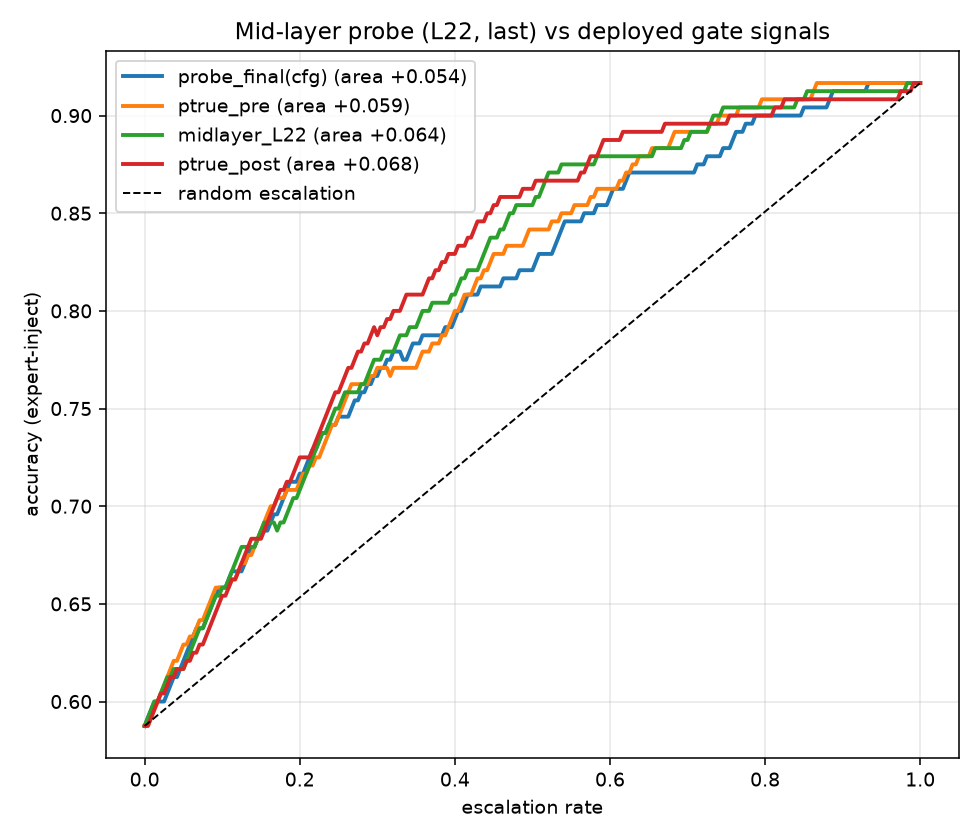
\includegraphics[width=.85\linewidth]{tradeoff_midlayer}
  \caption{Accuracy vs.\ escalation rate on the frozen test split for the
  mid-layer (L22) gate against final-layer probe and $\ptrue$ variants.}
  \label{fig:tradeoffmid}
\end{figure}

\section{Speech Input: Each Readout Has One Blind Modality}
\label{sec:speech}

\subsection{The late-layer cliff is text-input-specific}

Running the identical layer sweep on the TTS-rendered pool (audio input,
content unchanged): audio$\rightarrow$audio LOPO math reaches 0.93--0.96 at
mid-layers \emph{and the final layer does not invert} (L35 $=$ 0.936, vs.\
0.366 on text). A speak-mode template control
(\texttt{use\_tts\_template=True} on \emph{text} input) leaves the cliff
unchanged (L35 $=$ 0.362) --- the operative variable is the modality of the
\emph{input context} (text tokens vs.\ audio embeddings), not the output
mode. The duplex fine-tune re-purposed late-layer last-position processing
of text-token contexts specifically.

\subsection{Cross-modal transfer works --- for end-to-end models only}
\label{sec:xmodal}

Probes trained on text hidden states and scored on audio hidden states (and
vice versa) reveal where the representation becomes modality-shared: early
layers are modality-specific (0.54--0.60), and from $\sim$50\% depth
text$\rightarrow$audio transfer plateaus at 0.82--0.87 (0.855 at the
deployed L22) on MiniCPM-o~4.5. This replicates on MiniCPM-o~2.6 (onset
$\sim$46\% depth) and cross-family on Qwen2.5-Omni (onset $\sim$25\%). The
decisive control is \textbf{Freeze-Omni}: identical frozen Qwen2-7B weights
with audio attached via an adapter --- and cross-modal transfer is
$\approx$ dead (text$\rightarrow$audio 0.52--0.60, audio$\rightarrow$text
0.34--0.54). \textbf{The modality-shared mid-layer core is created by
training the backbone on the modality}; an adapter aligns well enough to
converse, but its audio-context hidden states live off the text manifold.
Practically: the cheap recipe ``calibrate the gate on text data, deploy on
speech'' is validated for end-to-end models and invalid for
adapter-attached ones.

\subsection{Verbalized introspection collapses on audio --- and why}
\label{sec:audioptrue}

The mirror-image failure: pre-answer $\ptrue$, robust on text
(\S\ref{sec:ptrue}), collapses under audio input on both MiniCPM duplex
generations, while both non-duplex controls stay intact
(Table~\ref{tab:audioptrue}).

\begin{table}[t]
\centering\small
\caption{Pre-answer introspection under audio input. Trap
$p_{\mathrm{yes}}$ is the mean stated probability of answering correctly on
a pool the model fails 100\% (lower is better-calibrated).}
\label{tab:audioptrue}
\begin{tabular}{llcc}
\toprule
model & FT type & trap $p_{\mathrm{yes}}$: text $\rightarrow$ audio & audio $\ptrue$-pre AUC \\
\midrule
MiniCPM-o 4.5 & duplex & .055 $\rightarrow$ \textbf{.556} (collapse) & .786 (trap dead) \\
MiniCPM-o 2.6 & duplex & .196 $\rightarrow$ .345 (compresses to $\sim$.5) & \textbf{.491} $\approx$ chance \\
Qwen2.5-Omni & omni-streaming & .279 $\rightarrow$ \textbf{.213} (intact) & .727 \\
Freeze-Omni & frozen + adapter & .165 $\rightarrow$ \textbf{.112} (intact) & (.612; capability caveat) \\
\bottomrule
\end{tabular}
\end{table}

Three controlled arms pin the mechanism on MiniCPM-o~4.5:
\begin{enumerate}
\item \emph{Not perception.} An ASR audit shows the model hears the trap
  questions fine (WER .074); $\ptrue$ computed on the model's \emph{own
  transcript} snaps back to .074 $\approx$ text; the well-heard subset still
  collapses (.582); corr(WER, $p_{\mathrm{yes}}$) $\approx$ 0.
\item \emph{Not a context prior or persona.} Irrelevant filler audio
  alongside the text question does \emph{not} inflate $p_{\mathrm{yes}}$
  (.001 --- it depresses it everywhere).
\item \emph{Binding.} Duplicating the question as text tokens alongside the
  audio fully restores introspection (.034). The verbal instance-check runs
  over \textbf{text-token pathways; audio embeddings do not feed it} ---
  while a linear probe reads the same instance information off the same
  forward pass at 0.93+.
\end{enumerate}
A log-odds decomposition agrees: the audio shift is graded (chat $+0.19$
$\rightarrow$ trap $+4.37$), i.e.\ on audio input verbal self-assessment
regresses to type-level priors. The failure also implies its own cheap fix,
confirmed twice: re-present the query as text (own transcript or
duplication) before asking --- ``repeat-then-judge.''

\subsection{Synthesis: four quadrants}
\label{sec:quadrants}

\begin{table}[t]
\centering\small
\caption{Mechanism synthesis across training regimes.}
\label{tab:quadrants}
\begin{tabular}{lcc}
\toprule
 & shared mid-layer core & faithful readouts \\
\midrule
raw text backbone & (text only) & \checkmark \\
omni-streaming e2e (Qwen2.5-Omni) & \checkmark built & \checkmark intact \\
\textbf{duplex e2e (MiniCPM-o $\times$2)} & \checkmark built & $\times$ overwritten (probe: late-layer/text; verbal: audio) \\
frozen backbone + adapter (Freeze-Omni) & $\times$ absent & \checkmark verbal survives (capability craters instead) \\
\bottomrule
\end{tabular}
\end{table}

End-to-end multimodal training \emph{builds} the shared semantic core;
duplex-style training additionally \emph{damages} the readouts;
omni-streaming gets both right; an adapter alone gets neither
(Table~\ref{tab:quadrants}). There is an elegant symmetry in the two
failures: the probe's readout is text-fragile and $\ptrue$'s readout is
audio-fragile --- in both cases the knowledge survives and a \emph{readout}
breaks, and in both cases the breakage is duplex-fine-tune-specific. For
gate design the consequence is concrete: \textbf{the mid-layer last-token
probe is the one signal that survives every quadrant that can converse.}

\section{The Gate as a System}
\label{sec:system}

\subsection{Accuracy--cost tradeoff}

On the frozen test split ($n=240$): small-only accuracy \textbf{0.588};
big-only (\texttt{gpt-5.5}) \textbf{0.917}; big relayed through the small
model's paraphrase 0.879 (relay tax 1--4 points). Every gate beats random
escalation at every operating point (Figure~\ref{fig:tradeoff}); the
balanced tier at a 33\% escalation budget reaches \textbf{0.779--0.787},
recovering $\sim$58\% of the small$\rightarrow$big gap at one third of the
big-only cost (\$1.12 per 100 queries big-only).

Figure~\ref{fig:tradeoff} also draws the baseline the type-shortcut audit
(\S\ref{sec:audit}) demands: a \emph{pool-oracle} router that escalates by
each pool's calibration-split base fail rate (true type labels, no
instance-level information, no test leakage). It captures $+0.042$ of the
gate's $+0.054$ area over random --- the system-level counterpart of the
AUC decomposition (0.715 of 0.821), and slightly harsher: in-distribution,
the instance-level residual the internal signal adds on top of type
routing is $+0.012$ area ($\sim$2 points at the balanced budget) --- not
significant at $n{=}240$ (paired bootstrap over test queries, $B{=}10^4$:
95\% CI $[-0.003, +0.027]$, two-sided $p{=}.13$); in distribution, the
gate is statistically on par with the pool oracle. The gate's case over
type routing therefore rests not on an in-distribution margin but on
transfer: the type shortcut is exactly what
collapses under LOPO (\S\ref{sec:audit}), while the mid-layer signal
survives it.

A \emph{trained} query-feature router closes this argument with data. We
fit a RouteLLM-style external router \citep{ong2024routellm} under
identical data conditions --- TF-IDF (word 1--2\,gram + character
3--5\,gram) $\to$ logistic regression on the calibration split's text
labels, seeing only the query surface. In-mix it lands \emph{below} even
the pool oracle (OOF AUC .669 vs.\ .715; tradeoff area $+.040$ vs.\ the
probe's $+.054$, mid-layer $+.064$, $\ptrue$-post $+.068$ on the same
test set and frozen expert answers); a 24-configuration sweep over
feature space and regularization tops out at .689, so the shipped
configuration is the query surface's ceiling, not a tuning artifact. Under LOPO it collapses entirely
(held-out-pool AUC .38--.57 vs.\ the mid-layer probe's .93 on math) and
its mean score on the 100\%-fail trap pool is .230 --- it \emph{misses}
the pool a router most needs to catch. The training receipt makes the
point starkly: at the argmax threshold the router's out-of-fold accuracy
on the calibration split, .678, \emph{exactly matches the majority-class
rate} (test .613 vs.\ majority .588) --- 360 queries of surface text buy
a weak ranking signal (train log-loss .38 vs.\ out-of-fold .59) and no
usable classifier. The internal probes pass the same accounting: at the
same threshold, same labels, and same logistic-regression machinery, the
text probe's out-of-fold accuracy is .772 (majority .678) and .779 on
test (majority .588), and the live audio mid-layer probe reaches
.764/.800 against .592/.512 --- real classifiers, not merely rankers;
the difference is purely the input representation
(Figure~\ref{fig:receipt}).

\begin{figure}[t]
  \centering
  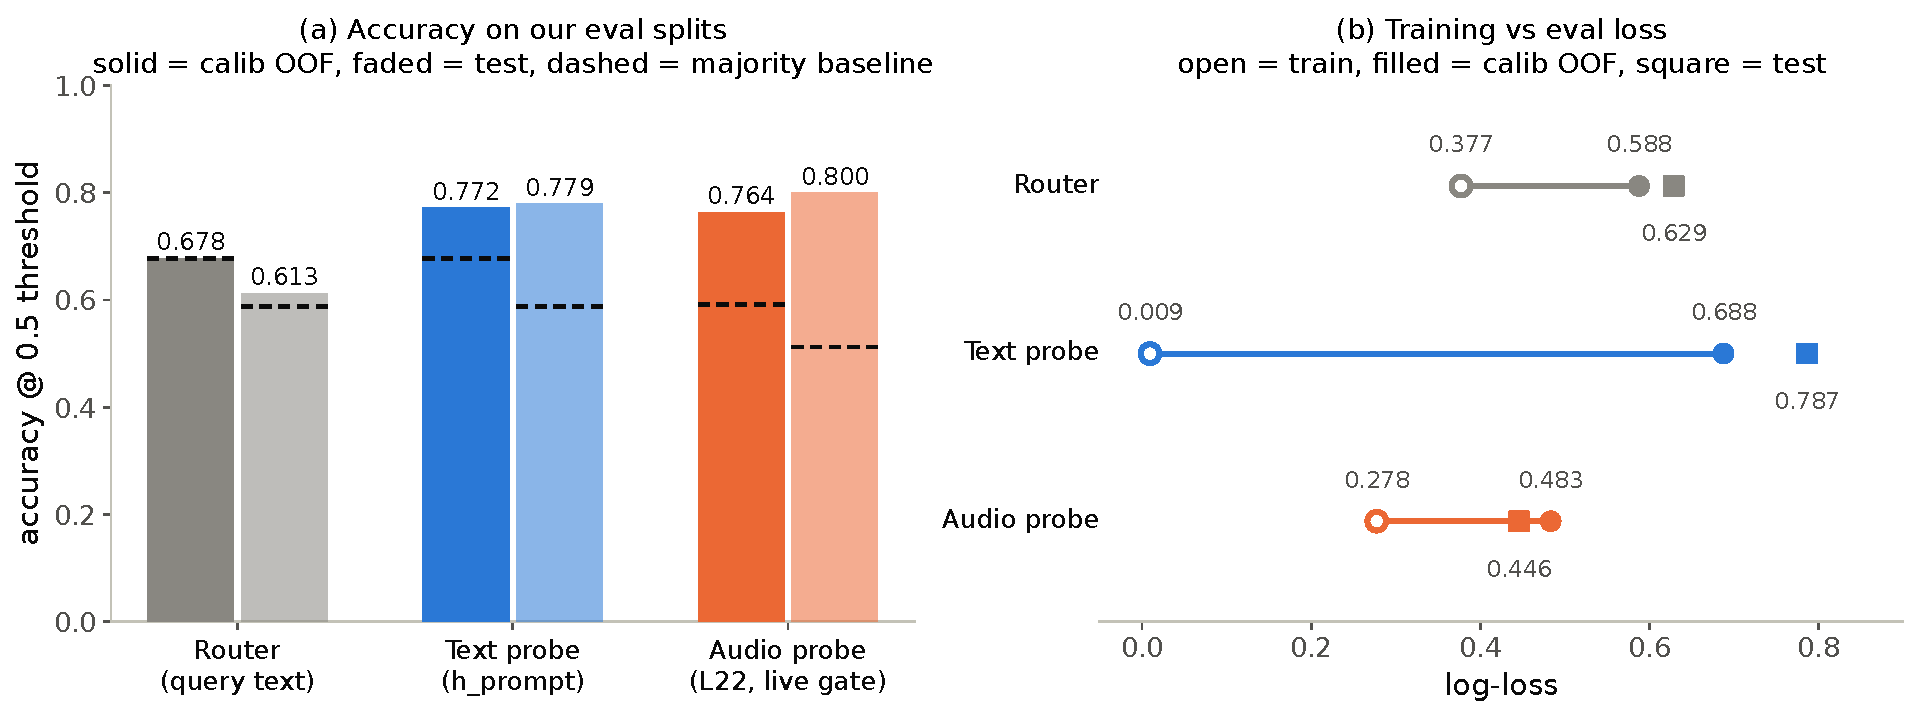
\includegraphics[width=\linewidth]{receipt_compare}
  \caption{The same training receipt for the external router and the two
  internal probes (identical labels, identical logistic-regression
  machinery). (a)~Accuracy at the 0.5 threshold on the calibration
  (out-of-fold) and frozen test splits, against each split's
  majority-class baseline (dashed): the router never clears majority;
  both probes clear it by 9--29 points. (b)~Train vs.\ eval log-loss:
  the audio probe generalizes cleanly (.278 train / .446 test, the
  best-calibrated signal); the text probe memorizes in-sample
  (4096 dims $\gg$ 360 queries) yet its held-out accuracy holds --- all
  reported numbers are out-of-fold or test.}
  \label{fig:receipt}
\end{figure}

Nor is the baseline data-starved. The identical recipe trained on
RouterBench \citep{hu2024routerbench} --- 36{,}497 public prompts,
routing \texttt{mixtral-8x7b} $\to$ \texttt{gpt-4} (escalation base rate
.432) --- reaches out-of-fold AUC .710 in-domain (accuracy .660 vs.\
majority .568; deferral area over random $+.033$): a hundred times the
data buys .04 of AUC, landing at our pool-oracle's level and still short
of the probe's .828. Its leave-one-benchmark-out transfer sits at chance
on the format-disjoint benchmarks (HellaSwag .502, GSM8K .509,
Winogrande .498), reproducing our LOPO collapse on public data, and our
calibration-trained router transfers to RouterBench \emph{below} chance
(AUC .440). The transfer failure is symmetric: RouteLLM's
\emph{released} preference-trained routers (BERT and
matrix-factorization, $\sim$100k GPT-4-vs-mixtral preference pairs),
scored zero-shot on our pool by their own inference code, reach test AUC
only .523/.533 --- below even the 360-sample same-data router --- and
both rank the 100\%-fail trap pool \emph{below} the ordinary hard pools.
The audio modality narrows but does not close the gap: against the live
gate's audio labels the same recipe reaches OOF AUC .743 / test .814
(gold text; the talker's own ASR transcript costs it only
$-$.005--.009) --- stronger than on text labels, because the audio
channel makes hard pools fail more uniformly and the type shortcut buys
more --- yet the audio mid-layer probe still leads every readout
(.843/.879 AUC, accuracy .800 vs.\ .696), and the router still requires
the full utterance plus transcription, so it cannot fire mid-stream.
Query-feature routing is the type shortcut and nothing else; the
standardized LLMRouterBench protocol \citep{llmrouterbench2026} remains
future work, but the information-source question is settled under
identical data, the ceiling replicates at $100\times$ the data on a
public benchmark, and routing knowledge fails to port across talkers in
either direction.

\begin{figure}[t]
  \centering
  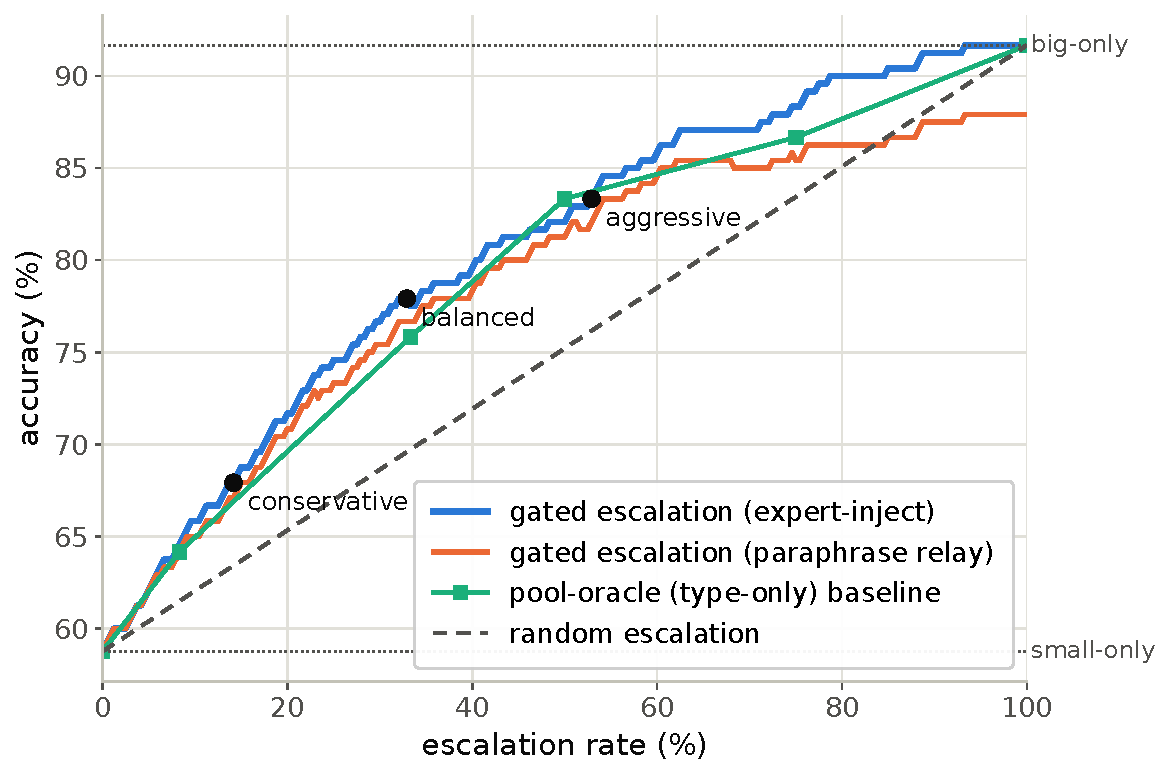
\includegraphics[width=.85\linewidth]{tradeoff}
  \caption{Accuracy vs.\ escalation rate, frozen test split: gated
  escalation vs.\ the random-escalation and pool-oracle (type-only)
  baselines between the small-only and big-only endpoints. The oracle
  captures most of the gate's in-distribution lift ($+0.042$ of $+0.054$
  area); the gate's advantage over type routing is transfer, not this
  margin (\S\ref{sec:audit}). See also Figure~\ref{fig:tradeoffptrue} for
  the $\ptrue$ variants.}
  \label{fig:tradeoff}
\end{figure}

\begin{figure}[t]
  \centering
  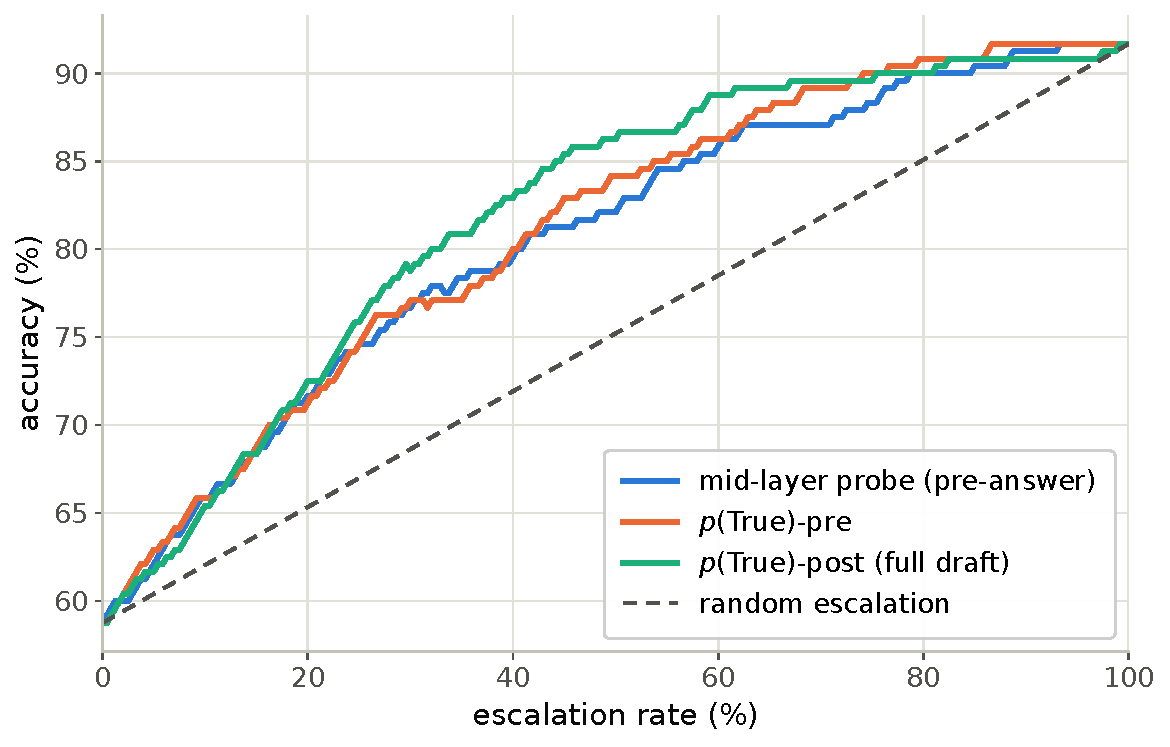
\includegraphics[width=.85\linewidth]{tradeoff_ptrue}
  \caption{Same tradeoff for the $\ptrue$ signals (pre-answer and
  post-draft).}
  \label{fig:tradeoffptrue}
\end{figure}

\subsection{Against the model's own thinking mode}
\label{sec:thinking}

MiniCPM-o~4.5 ships a built-in \texttt{enable\_thinking} reasoning mode ---
self-escalation in place. Table~\ref{tab:policy} compares deployment
policies with measured latencies. \textbf{Gated-cloud escalation dominates
all-THINK on both axes at every escalation rate.} The reason is mechanistic,
not incidental: the gate predominantly flags knowledge/trap failures, which
thinking cannot fix --- thinking helps math (fail .187 $\rightarrow$ .127)
but \emph{hurts} chat (.207 $\rightarrow$ .233) --- so external escalation
is necessary, not merely better.

\begin{table}[t]
\centering\small
\caption{Policy table, frozen test split ($n=240$). Latency from per-pool
measured medians; think and cloud latencies per-query.}
\label{tab:policy}
\begin{tabular}{lcccc}
\toprule
policy & acc & lat.\ mean (s) & P50 & P95 \\
\midrule
fast-only & .588 & 3.0 & 3.5 & 4.2 \\
all-THINK (o4.5's own) & .637 & 22.4 & 17.2 & 60.1 \\
gated-think @.33 & .613 & 12.1 & 3.6 & 47.6 \\
gated-cloud @.15 & .688 & 5.3 & 3.6 & 10.1 \\
\textbf{gated-cloud @.33} & \textbf{.787} & \textbf{6.5} & 3.6 & 20.8 \\
gated-cloud @.50 & .858 & 7.0 & 3.6 & 24.4 \\
\bottomrule
\end{tabular}
\end{table}

\subsection{The fork: deciding before the first token}
\label{sec:fork}

The mid-layer probe is one 4096-d dot product on a hidden state the forward
pass already computes: forking a decision branch at layer $k$ costs
microseconds and never stalls the main forward. The design question is at
which depth the signal is sufficient. Measured on H100 (CUDA-synchronized,
truncated-forward): the L22 decision lands in \textbf{20\,ms (text) /
45\,ms (audio)}, vs.\ time-to-first-token of 36 / 68\,ms --- the decision
exists \emph{before decoding starts} and sits far inside the 200--300\,ms
turn-taking budget \citep{stivers2009universals}. Per-layer curves
(Figure~\ref{fig:fork}) show L22's hidden state is available at 57\% of
prefill wall-time (61\% audio) while L22 is simultaneously the in-mix
quality peak (OOF .866 $>$ final layer .835): deciding early costs nothing,
and the cloud call can launch while the remaining $\sim$40\% of prefill
plus the whole decode still runs. Forking much earlier is not free:
pre-50\%-depth layers are both weaker (L10 $\approx$ .794) and
modality-specific (\S\ref{sec:xmodal}); the fork belongs at $\sim$55--60\%
depth. For comparison, $\ptrue$-pre costs 39 / 67\,ms (an extra short
prefill) and $\ptrue$-post costs a full draft (1.9 / 3.5\,s).

\begin{figure}[t]
  \centering
  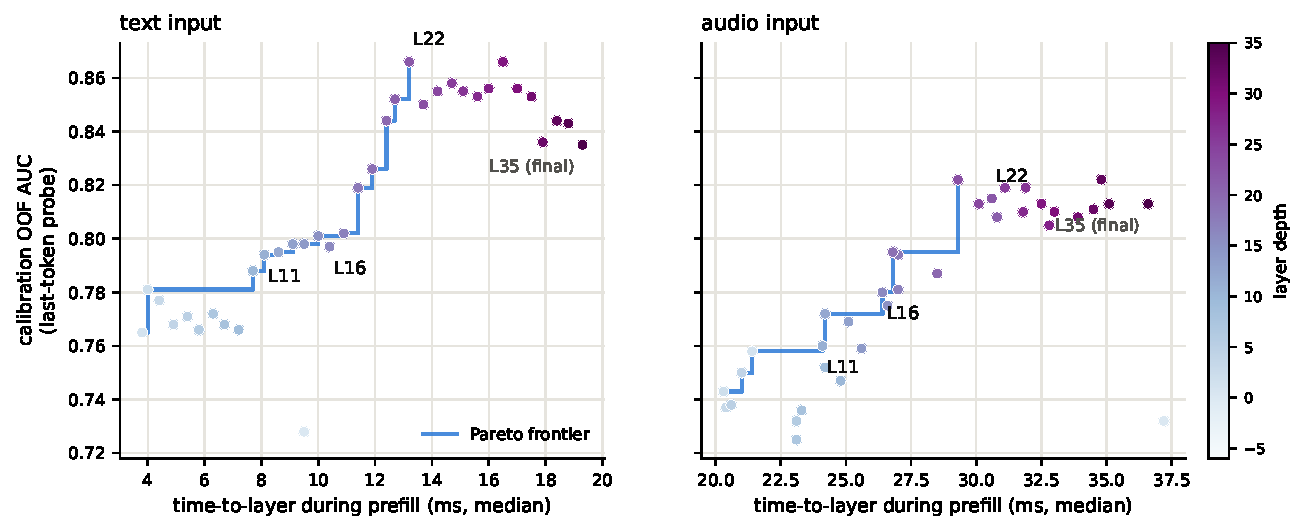
\includegraphics[width=.85\linewidth]{fork_pareto}
  \caption{Fork-depth Pareto: per-layer truncated-forward wall-time vs.\
  gate quality. The deployed L22 sits at the quality peak while its hidden
  state is available at $\sim$57--61\% of prefill wall-time.}
  \label{fig:fork}
\end{figure}

\subsection{Does the cloud round-trip hide inside the talker's floor time?}
\label{sec:overlap}

If the gate fires at prefill and the cloud call launches immediately, the
expert result is ready before the local answer finishes speaking for
40--58\% of the whole test mix (audio input buys more time than text). But
\emph{gate-escalated} queries skew toward short local answers (trap and
knowledge pools; trap overlap $\approx$ 0), so pure overlap covers only
$\sim$20--31\% of escalations at a 33\% budget (Figure~\ref{fig:overlap}).
The residual wait after the local answer ends is P50 2--3\,s --- one stall
sentence --- but P90 $\sim$27\,s, dominated by the expert's own reasoning
latency. This argues for a fast-expert tier or streamed partial results in
step 2, and it quantifies the stall-phrase budget an injection protocol
must cover.

\begin{figure}[t]
  \centering
  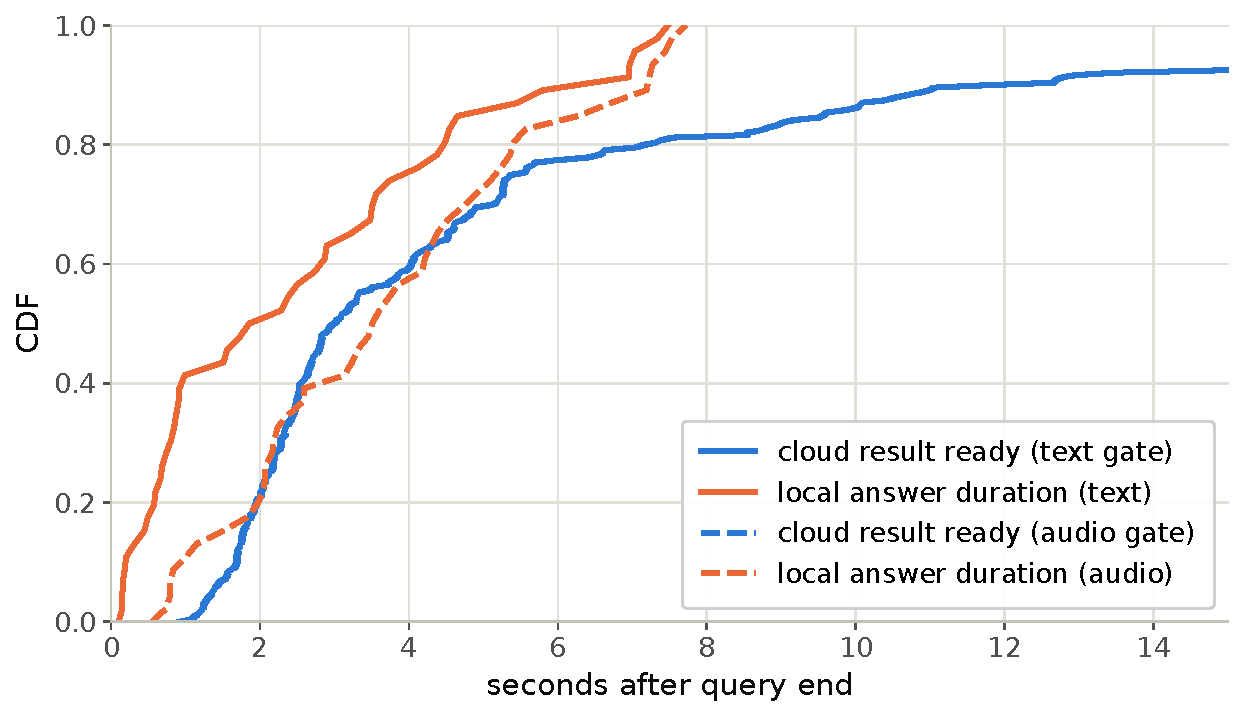
\includegraphics[width=.85\linewidth]{overlap}
  \caption{Cloud round-trip vs.\ local answer duration: probability the
  expert result arrives before the local answer ends (+slack), whole mix
  and gate-escalated subset, text and audio.}
  \label{fig:overlap}
\end{figure}

\section{Results}
\label{sec:results}

% Main results table (tab:transfer) is declared in signal.tex so it
% floats to an early page.

\subsection{Live escalation}
\label{sec:live}
\label{sec:liveloop}
\label{sec:livecurve}

We ran the 240 frozen test queries through four escalation tiers,
each a complete turn-based loop with audio input
(\S\ref{sec:liveproto}). The primary sweep retains the model's output
as text; a separate run of the balanced tier with speech synthesis
enabled leaves all 84/240 gate decisions unchanged and measures
speech onset. We score deployed-channel answer accuracy: the
correctness of the relayed content after the full system path.
Headline numbers use a pre-registered input filter that removes 21
formula-LaTeX queries and one broken recording, because the speech
rendering destroys the symbolic input before the model receives it.
Accuracy rises monotonically,
$\mathbf{42.2\% \to 52.8\% \to 59.2\% \to 63.3\%}$ at 0/14/31/57\%
escalation, and every tier's gain is significant (paired bootstrap;
Table~\ref{tab:transfer}, Figure~\ref{fig:dualview}). The gate also
exceeds matched-rate random
escalation at every tier: by 7.2--9.4 points on deployed-channel
accuracy, and by 5.3--8.3 points when the relay channel is factored
out (Figure~\ref{fig:dualview}).

% fig:dualview is declared at the end of Section 4 so it floats
% onto the page where these results are discussed.

A measured always-escalate arm reaches 66.5\%. The gain from 57\% to
100\% escalation is small because the expert sees the model's own
transcription: the same sessions reach 92.2\% when the expert
receives the reference transcript, so the transcription channel, not
selection, is the limit at high escalation rates. Live accuracies
have a replication floor of $\pm$2--3 points; no claim rests on a
smaller difference. Full tables, latency profiles, and boundary cases
are in Appendix~\ref{app:livedetail}.

\paragraph{Serving-regime checks.}
Replaying the loop with the talker enabled leaves the frozen ranking
nearly unchanged (AUC 0.871/0.856 versus 0.866 with the talker
disabled). A teacher-forced concurrent-prefill variant is less stable
and requires an in-regime refit; its external results remain
exploratory (Appendix~\ref{app:duplexval}). Under the model's native
full-duplex head, the read moves to the head's own listen$\to$speak
commit point, and the probe is refit in regime on a widened
5{,}228-row calibration merge under the official serving
configuration, with labels judged on the native answers. The refit
reads at AUC 0.876 internally and 0.771 on the four English external
QA pools. The Mandarin reasoning pool is lower, at 0.621; a
1{,}500-question held-out Mandarin set of facts, knowledge, and
commonsense reads at 0.811, so the gap is multi-step reasoning
rather than language (Appendix~\ref{app:native}). Re-mixing the
native gate's decisions with cached expert outcomes beats
matched-rate random on all five English pools at both deployed
tiers; with per-language thresholds the Mandarin pool escalates at
the nominal rates and beats matched-rate random at the two lower
tiers. A full native live run on the internal 240 queries, under the
earlier inherited serving configuration, improves accuracy from
0.371 to 0.537 at 45\% escalation, below the prediction of 0.596
from the same re-mix arithmetic, because relaying the returned
answer is lossy. These checks support the ranking beyond the primary
turn-based loop, but they also show that read points, probe weights,
and thresholds must be calibrated for the serving regime
(Appendix~\ref{app:native}).

\section{Discussion}
\label{sec:discussion}

\subsection{Design consequences: the two-stage gate}

The evidence converges on a two-stage design:
\begin{itemize}
\item \textbf{Stage 1 (prefill, effectively free):} a mid-layer
  ($\sim$60\% depth) last-token probe --- 20/45\,ms, before the first
  token, and the only signal that survives duplex fine-tuning \emph{and}
  both input modalities (\S\ref{sec:quadrants}). Open engineering item:
  score-scale calibration for threshold (rate) transfer.
\item \textbf{Stage 2 (optional, post-draft):} $\ptrue$-post on the drafted
  answer --- the strongest single signal (0.899); the draft doubles as the
  distilled escalation query and as the fallback answer. On audio input,
  never ask over raw audio context: run $\ptrue$ on the model's own
  transcript (``repeat-then-judge,'' \S\ref{sec:audioptrue}).
\end{itemize}

\subsection{Positioning vs.\ query-side routing}

Query-side routers \citep{ong2024routellm,ding2024hybrid,chen2023frugalgpt}
decide before generation from query features, and the big model then
answers the user directly. Neither transfers to full-duplex voice: the user
talks to one voice whose session state lives in the small model, and
query-side features are precisely the ``type shortcut'' our audit
quantifies (pool oracle 0.715 vs.\ probe 0.822 in-distribution) and LOPO
breaks. The signal must come from the answering model itself --- consistent
with \citet{llmrouterbench2026}'s attribution of router failures to
model-recall gaps. A head-to-head comparison of query-feature routers vs.\
internal-signal gates under distribution shift, on their standardized
protocol, is natural future work.

\subsection{Step 2 preview: result injection}

Step 2 --- returning the thinker's result into the live duplex session ---
is scoped by our data. The official streaming interface exposes a per-chunk
text-injection point (\texttt{teacher\_forcing\_text}), and our streaming
smoke test surfaced the first substantive obstacle: the talker
\emph{pushes back} on injected expert results that conflict with its own
reasoning rather than relaying them --- injection protocol and authority
framing are a research problem, not plumbing. The overlap analysis
(\S\ref{sec:overlap}) sets the timing budget: P50 one stall sentence; P90
dominated by expert latency, arguing for a fast-expert tier or streamed
partial results.

\subsection{Limitations}
\label{sec:limitations}

(i) $\ptrue$ prompt sensitivity: one phrasing each (pre/post).
(ii) The audio arm is single-voice TTS speech; SD-QA real-speech validation
is open. (iii) Mid-layer probe threshold transfer needs deployment-grade
calibration; AUC/area claims are unaffected. (iv) The audio side of the
introspection-collapse finding is MiniCPM-scoped (two generations of one
family); a new open-weight full-duplex family is a pre-registered
prediction test --- it should show the late-layer text-input cliff.
(v) The frozen test split is reused across signal comparisons (signals were
pre-specified; a fresh test set would be cleaner). (vi) Labels come from a
single judge family, bounded by a stronger re-judge (deltas $\le$0.010) but
without human labels.

\section{Conclusion}
\label{sec:conclusion}

Zero-training self-knowledge in a small full-duplex model exists, is
strong, and is modality- and layer-fragile in systematic,
duplex-fine-tune-induced ways. The standard readouts --- final-layer probes
and verbalized self-evaluation --- each have one blind modality, and both
blind spots are created by the duplex fine-tune; the mid-layer
representation underneath survives everything we tested. Read there, the
resulting gate decides before the first output token, transfers from cheap
text calibration to speech on end-to-end models, and as a system dominates
the model's own thinking mode on both accuracy and latency. Step 2 ---
getting the thinker's answer back into the talker's mouth --- is where this
program goes next.


\bibliographystyle{plainnat}
\bibliography{refs}

\clearpage
\appendix
% =========================================================================
% Working TODO / roadmap — DELETE THIS SECTION BEFORE SUBMISSION.
% Experiment-level items mirror RESULTS.md / TECHNICAL_REPORT.md §9.
% =========================================================================
\section*{TODO / Roadmap (working section --- delete before submission)}
\label{sec:todo}

\subsection*{Experiments}
\begin{itemize}
\item \todonote{SD-QA arm B: validate the audio findings on real (dialectal)
  speech instead of single-voice TTS \citep{faisal2021sdqa}}
\item \todonote{mid-layer probe threshold-transfer calibration
  (Phase-3-style C-compression) --- needed for deployment claims, not for
  AUC/area claims}
\item \todonote{pre-registered prediction test: when a new open-weight
  full-duplex family lands (e.g.\ Qwen3.5-Omni-class), it should show the
  late-layer text-input cliff}
\item \todonote{$\ptrue$ prompt-sensitivity sweep (currently one phrasing
  each for pre/post)}
\item \todonote{head-to-head query-feature router vs.\ internal-signal gate
  under distribution shift on the LLMRouterBench protocol; NEAR-TERM
  (decided 2026-07-30): add an offline query-feature router baseline
  (text-only classifier over the query surface, $\sim$\$10) as a line in
  the tradeoff figure --- closes the ``type recognition is all you need''
  objection with data (expected: matches the pool-oracle component
  in-mix, collapses under LOPO); no live arm --- external routing needs
  the full query + ASR and structurally cannot fire mid-utterance
  (one-sentence annotation on the live figure instead). OFFLINE BASELINE
  DONE (2026-07-30, RESULTS.md \S 8f, \$0): TF-IDF+LR router in-mix OOF
  AUC .669 $<$ pool-oracle .715, area $+.040$ (worst of all signals);
  LOPO collapse .38--.57, trap mean score .230. WRITTEN into
  \S\ref{sec:system}; LLMRouterBench protocol comparison stays future
  work}
\item \todonote{step 2: injection protocol + authority framing (talker
  pushes back on conflicting expert results); fast-expert tier or streamed
  partial results for the P90 tail. DONE (2026-07-30, RESULTS.md \S 8b,
  172 sessions, $\sim$\$6): (1) deployed channel clean --- model-wrong
  $\times$ correct-inject comply $=1.00$ ($n{=}24$), the live curve is
  uncontaminated; (2) L0 hypothesis CONFIRMED --- comply rises
  $.42 \to .75$ across gate-score quartiles, resistance $.25$ vs $.08$:
  the same signal that triggers escalation predicts relay compliance;
  (3) worst-case framing ladder: neutral $.00$ / deployed authority
  $.53$ / strong-override $.79$ / assistant-seeding BACKFIRES ($.25$
  comply, $.62$ lip-service --- the model walks back its own forced
  speech); (4) silent-override on math: the model re-derives instead of
  relaying or disputing (bare numbers carry no authority against its own
  computation chain); (5) swallow rate $.64$ when unconfident --- expert
  quality is the accuracy ceiling. Decision: keep the deployed F1
  authority framing for the full sweep; strong-override stays shelved
  (would plausibly raise the swallow rate). WRITTEN into
  \S\ref{sec:inject} (2026-07-30)}
\item \todonote{Part-2 acceptance decided (2026-07-30 grilling): paper-grade
  \emph{live} tradeoff curve (heard-accuracy, 240 test queries $\times$ 3
  tiers + never/always-escalate endpoints, bootstrap CIs, offline audio
  curve as reference). Gate redesign for the streaming trap miss (a
  full-duplex-specific read-position failure: short audio, entity in the
  zero-padded tail chunk; live 1/5 vs offline $\approx$ full catch):
  end-of-turn read becomes the \emph{deciding} gate (pre-TTFT, 45\,ms $<$
  68\,ms TTFT; escalation rate calibrated on this single score), mid-stream
  chunk gate demoted to speculative expert prefetch with end-of-turn veto
  (abort/ignore the expert on veto). VALIDATED (2026-07-30, RESULTS.md
  \S 8c): the streaming end-of-turn read (single-space assistant prefill,
  L22 at assistant-start) reaches AUC .887 --- above the offline .843
  reference --- and trap fire@balanced recovers .20 $\to$ .90; thresholds
  in \texttt{midlayer\_gate\_audio.json}. Prefetch subsequently RETIRED
  (see the speculative-execution entry): the end-of-turn read is the only
  gate; the expert starts at end of turn. FULL SWEEP DONE (2026-07-30,
  RESULTS.md \S 8e + \texttt{live\_dualview}): four live arms never
  .400 / cons 14\% .446 / bal 35\% .529 / aggr 55\% .633; paired
  bootstrap on frozen \texttt{gated\_traces\_v2.parquet} --- bal/aggr
  deltas significant, conservative $+.046$ n.s.; dual-view figure
  (honest heard-acc + gold-inject counterfactual, channel cost
  $+.05/+.11/+.13$ all significant) replaces the offline-audio-reference
  plan; always-live arm cancelled (synthesized from frozen gold, \$0).
  WRITTEN into \S\ref{sec:live}}
\item \todonote{dead-air fix decided (2026-07-30 grilling): deadline-aware
  expert effort selection, not blanket effort=low. Measure the two
  governing dimensions: (1) expert latency as a function of effort
  $\times$ query type (escalated subset $\times$ \{low, high\}, $\sim$200
  calls, probation-throttled); (2) difficulty operationalized as
  effort-sensitivity $\Delta$acc(high$-$low) per pool — predicted
  $\approx 0$ for trap (retrieval-bound) vs.\ large for math
  (execution-bound), mirroring the 6c talker-side think-gain structure
  (potential cross-scale finding: extra compute rescues execution
  failures, not retrieval failures). Policy conditions only on the
  observable time budget (remaining audio + filler tolerance), never on
  query type. Offline replay simulation of dead-air CDF under
  fixed-high / fixed-low / deadline-aware precedes any live change;
  streamed partials rejected (latency is pre-token hidden reasoning),
  speculative laddering deferred (probation call volume). MEASURED AND
  RESOLVED (2026-07-30, RESULTS.md \S 8d): effort tax $\approx 0$
  everywhere \emph{including gold math} (low 1.00 = med 1.00) --- the
  effort-sensitivity prediction is REFUTED; latency doubles at medium
  (P50 5.8$\to$9.1\,s, P95 23.9$\to$78.8\,s) $\to$ \textbf{fixed-low
  ships}; deadline-aware collapses to the simplest policy. Escalated
  failures are knowledge-bound at both scales (cross-scale finding with
  6c). WRITTEN into \S\ref{sec:liveloop}}
\item \todonote{expert-pipeline oracle removal (2026-07-30 grilling):
  (1) query form decided --- talker self-transcription at fire time
  (fork the streaming session), replacing the dataset gold text; shares
  the same $\sim$200-call batch as the effort characterization (transcript
  queries $\times$ \{low, high\} vs.\ frozen gold-text high-effort
  answers = ASR-distill tax + effort tax in one batch; methodology
  lineage: SD-QA / HeySQuAD paired gold-vs-ASR arms). WER risk
  concentrated on hard-knowledge (.224). (2) prefetch realism decided ---
  milestone 1 sent the \emph{full} question text at 27--40\% of the
  audio (a deployment-impossible oracle inflating the 5/6 overlap
  result). Fix framed as \emph{query-level speculative execution}
  (speculative decoding's draft--verify--rollback skeleton at sentence
  granularity; lossy, unlike token-level): measure the wait-k-style
  completeness curve first (calib texts truncated at 25/50/75\% of
  audio progress, mini-judge scores ``answerable core already
  spoken?'', $<$\$1) = the acceptance rate. MEASURED (2026-07-30,
  RESULTS.md \S 8c): acceptance .07/.19/.51 at 25/50/75\% --- LOW ---
  so prefetch is dropped per the pre-agreed rule; the curve goes in the
  paper as the negative-result explanation, and trap's floor
  (.00/.10/.27) unifies with the probe's trap signal-placement failure
  (same back-loaded-core property, measured twice).
  ASR-DISTILL TAX MEASURED (2026-07-30, RESULTS.md \S 8d): expert on
  self-transcripts .57 vs gold .85 on the escalated population; math
  $-$.70 mostly a TTS-of-LaTeX artifact (scope note: audio arm evaluates
  speakable content); deployment-real residue = knowledge entities
  $-$.31; rescues negative (robust prompt no-op, $k$-best GER trades
  trap $+.06$ for knowledge $-$.12), Whisper recovers only .62 of the
  .82 ceiling $\to$ channel-inherent. USER SCOPE DECISION: ASR is a
  channel property, not a contribution --- handled via the dual-view
  curve; ASR robustness cited as orthogonal work. WRITTEN into
  \S\ref{sec:livecurve}.
  Rejected with rationale: micro-turn streaming of the question (saves
  only transmission+prefill $\approx$0.15\,s of a 30-token query;
  reasoning cannot start before semantic completeness), literal
  speculative decoding (provider-internal, no API handle; talker decode
  not a bottleneck), draft-then-verify expert (verifying a fact
  $\approx$ retrieving it for retrieval-bound escalations). Future
  work: tool-using expert could do speculative retrieval off partial
  input; Moshi inner-monologue as architectural reference for
  transcript-so-far}
\item \todonote{fresh test split for final camera-ready numbers (current
  test split reused across signal comparisons)}
\item \todonote{statistics hardening (2026-07-26 Notion review): DeLong
  paired tests for same-test-set signal comparisons; McNemar / paired
  bootstrap for the paired text-vs-audio fail-rate deltas; paired bootstrap
  for the gate-vs-pool-oracle tradeoff residual (+0.012 area, added
  2026-07-29 — likely within noise at $n=240$, must be tested before any
  claim rests on it). PARTIAL (2026-07-30): live-arm paired bootstrap
  DONE (\texttt{live\_dualview}, Table~\ref{tab:live}); the rest still
  open; expand pools to
  500--1000 each from the same public benchmarks (GSM8K test, MMLU-Pro,
  TriviaQA, SimpleQA have headroom) + extra benchmark families for
  diversity (GPQA/ARC for knowledge, NQ for fact) + remaining 10 SD-QA
  dialect splits}
\item \todonote{injection payload budget (2026-07-30 discussion): current
  note is tiny (template + low-effort answer P99 $\approx$150 tokens vs a
  32k-class window; deployed low-effort answers are P50 3 words), so no
  near wall --- but two scaling paths identified. (1) Session audio
  itself hits the window first ($\sim$18 tok/s $\Rightarrow$ $\sim$30 min
  fills 32k) --- a generic long-lived-duplex limitation, not an
  injection-mechanism issue. (2) Long-form expert outputs (documents,
  derivations, tool results): principle = KV holds only what will be
  \emph{spoken} (voice bounds the useful payload at 2--4 sentences);
  full output stays in the external answer cache; follow-up questions
  page further notes in across turns (paging, not intra-turn dribbling).
  Open \$5-scale experiment: does ``answer + one-sentence justification''
  restore math relay compliance (the silent-override finding says bare
  numbers lack authority --- authority wants more tokens, capacity wants
  fewer; find the knee)}
\item \todonote{closed-source behavioral arm (2026-07-26 Notion review):
  trap $p_\mathrm{yes}$ text vs.\ audio + modality tax on audio-capable
  commercial APIs (GPT audio / Gemini Live) with the existing 600 wavs;
  probes impossible (no hidden states); if the API exposes no logprobs,
  estimate $p_\mathrm{yes}$ by sampling Yes/No $k$ times}
\end{itemize}

\subsection*{Writing / assets}
\begin{itemize}
\item \todonote{discussion-section frame (2026-07-30, user's schoolkid
  analogy): three failure species $\times$ perceivability —
  retrieval-type (``don't know XYZ'': the empty lookup is an observable
  event $\to$ pre-answer signals work; trap fire .90), execution-type
  (``stuck mid-solution'' $\to$ decode-time entropy works; math
  entropy@16 .860), metacognitive-type (``doesn't know the question has
  a trap'', Goldbach-to-a-schoolkid: no failure event occurs in the
  model's experience $\to$ all signals blind; FalseQA fire .18, no score
  separation). Parallels human feeling-of-knowing literature (accurate
  for memory retrieval, overconfident for insight problems). Explains
  the two-stage gate architecture and why query-surface routers also
  miss species 3. RESULTS \S 8g. WRITTEN into the discussion
  (three-species subsection) + \S\ref{sec:falseqa} (2026-07-30)}
\end{itemize}
\begin{itemize}
\item \todonote{affiliations, emails, author order + contribution notes on
  the title page}
\item \todonote{regenerate \texttt{concept\_probe\_vs\_ppl} figure with
  English labels (Fig.~\ref{fig:concept})}
\item \todonote{regenerate ROC figure to include $\ptrue$ curves
  (Fig.~\ref{fig:roc})}
\item \todonote{verify the \citet{llmrouterbench2026} bib entry (authors /
  exact title, arXiv:2601.07206) and the MiniCPM-o 4.5 model-card entry}
\item \todonote{decide target venue + switch template (currently generic
  preprint article); candidates: ICASSP/Interspeech (speech systems) vs.\
  ACL/NeurIPS (LM analysis)}
\item \todonote{bootstrap CIs are computed for headline numbers in
  RESULTS.md --- surface them in tables beyond Table~\ref{tab:rq1}}
\item \todonote{appendix: full per-pool tables, judge prompts, $\ptrue$
  prompts, reproducibility statement (seeds, pins, spend)}
\end{itemize}


\end{document}
